\documentclass[main.tex]{subfiles}
\ifxetex\else\onlyinsubfile{\usepackage{CJKutf8}}\fi
\begin{document}
\ifxetex\else\begin{CJK*}{UTF8}{song}\fi

\chapter{中断处理}
%% my chapter 1 content
%\onlyinsubfile{this only appears if chapter1.tex is compiled (not when main.tex is compiled)}
%\notinsubfile{this only appears if main.tex is compiled (not when chapter1.tex is compiled)}
%% more of my chapter 1 content
%%
\section{介绍}
ARM提供了7种运行模式,分别是 user、 system、 supervisor、 IRQ、 FIQ、 abort、 undefined。除了 user模式外,其他6种模式都是特权模式,如图\ref{figure:3-1}所示。

\begin{figure}[htp]
\centering
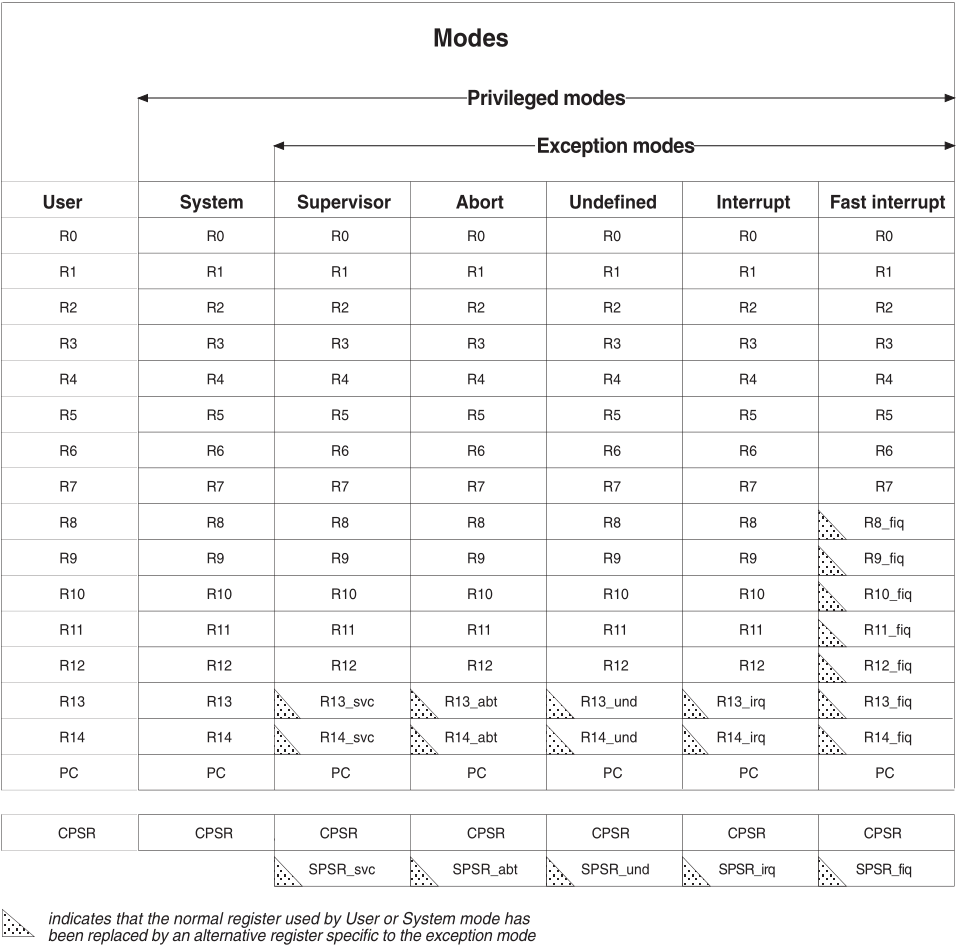
\includegraphics[scale=0.5]{figures/3-1.png}
\caption{ARM的7种模式}
\label{figure:3-1}
\end{figure}

\begin{itemize}
\item User : 唯一的非特权模式,用户程序运行在这种模式
\item System:与用户模式一样,只是属于特权模式
\item Supervisor:操作系统内核运行的模式,当 CPU复位或 swi指令执行时进入这种模式
\item IRQ :   当一个普通中断产生时将会进入这种模式
\item FIQ :   当一个快速中断产生时将会进入这种模式
\item Abort : 当 CPU访问内存出现异常时将会进入这种模式
\item Undefined : 当 CPU执行未定义指令时会进入这种模式
\end{itemize}

当ARM进入到异常模式时,它会跳转到从0开始的几个固定地址开始执行,这几个固定的地址称为异常向量表,如图\ref{figure:3-2}所示。该表共有8项,当 CPU遇到异常,就会跳转到相对应的地址开始执行。

\par
本章主要关注的异常类型是 IRQ。当外部设备触发中断时, ARM会把模式设置为 IRQ模式,然后将 pc设为 0x18。此时, SPSR\_\-irq=CPSR, r14\_\-irq=(中断返回地址+4)。

\begin{figure}[htp]
\centering
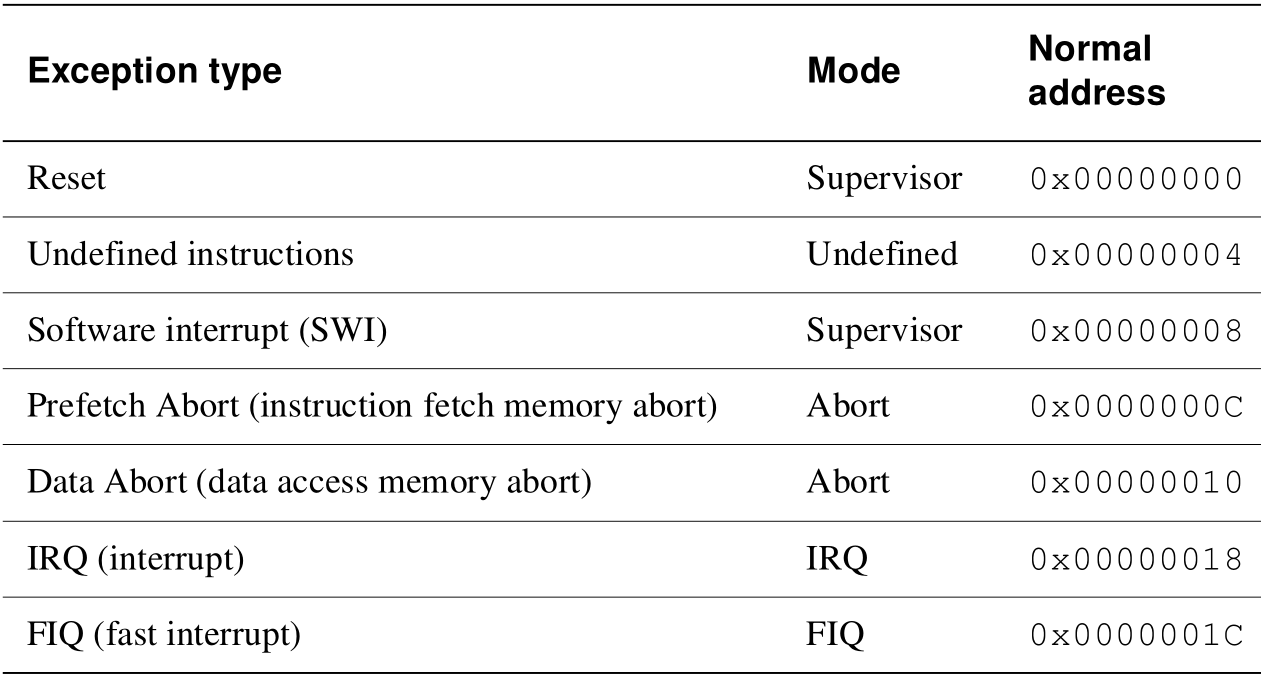
\includegraphics[scale=0.35]{figures/3-2.png}
\caption{ARM的异常}
\label{figure:3-2}
\end{figure}

\section{扩充entry.S}
我们要对entry.S进行扩充以满足中断处理的需要。扩充的内容有以下三个方面:
\begin{itemize}
\item 填充异常向量表。
\item 初始化C语言中未初始化的全局或者静态变量。
\item 初始化各个 CPU模式的栈。
\end{itemize}

首先来填充异常向量表,如代码\ref{code:3-1}所示。

\begin{code}
\captionof{listing}{chapter03/kernel/entry.S}
\label{code:3-1}
\inputminted[firstline=73,lastline=104,linenos,numbersep=5pt,frame=lines,framesep=2mm]{gas}{src/chapter03/kernel/entry.S}
\end{code}

可以看出,真正有效的只有 reset和 irq两项。因为 kernel.img被加载到 0x8000这个地址,从 \_entry开始的异常向量表位于 0x8000,而 CPU希望异常向量表在0地址。因此,我们要把异常向量表从 0x8000复制到 0地址,才能保证异常的正常处理。复制异常向量表如代码\ref{code:3-2}所示。

\begin{code}
\captionof{listing}{chapter03/kernel/entry.S}
\label{code:3-2}
\inputminted[firstline=106,lastline=112,linenos,numbersep=5pt,frame=lines,framesep=2mm]{gas}{src/chapter03/kernel/entry.S}
\end{code}

在C语言中,要把未初始化的全局或静态变量全部置0。编译器会把这些变量统一放在一个称为 BSS(Block Started by Symbol)的段中。在链接器脚本 kernel.ld.in(代码\ref{code:2-5})中,我们定义的两个符号 \_edata和 \_end,分别标识了 BSS段的开始和结束。在调用C程序之前,要确保这部分变量的值是0。这正是代码\ref{code:3-3}的功能。

\begin{code}
\captionof{listing}{chapter03/kernel/entry.S}
\label{code:3-3}
\inputminted[firstline=114,lastline=123,linenos,numbersep=5pt,frame=lines,framesep=2mm]{gas}{src/chapter03/kernel/entry.S}
\end{code}

接下来,为各个异常模式设置栈。记住,当前 CPU正运行在 supervisor模式。我们按照顺序先后为 undefined、 abort、 IRQ和 supervisor模式设置了栈。我们只给 undefined、 abort和 IRQ的栈分配了 12个字节。后面我们会看到, 12个字节就够了。 Supervisor的栈稍微大一点,从 (0x1000-36)开始往0地址延伸。
\begin{code}
\captionof{listing}{chapter03/kernel/entry.S}
\label{code:3-4}
\inputminted[firstline=125,lastline=142,linenos,numbersep=5pt,frame=lines,framesep=2mm]{gas}{src/chapter03/kernel/entry.S}
\end{code}

在实际应用中,绝大部分代码运行在两种模式: user和 supervisor模式。 User模式用于运行用户应用程序, supervisor模式用于运行操作系统内核。
\par
当系统发生异常时,我们完成一些准备工作后,切换到 supervisor模式,然后在 supervisor模式下完成后续的流程。

\section{保存中断现场}
所谓中断现场 (context),是指在中断发生前CPU的运行状态,即所有寄存器的值。前面讲过,当 CPU被外部设备中断时,它会自动将 pc=0x18, SPSR\_\-irq=CPSR, r14\_\-irq=(中断返回地址 +4),其他寄存器仍然保持中断发生前的状态。因为在后续处理中断过程中可能会修改这些寄存器的值,我们必须完整地保存中断发生前 CPU的运行状态,这个过程称为保存现场。当中断处理完成后,把这些保存的值恢复到寄存器中, CPU将以中断发生前的状态继续运行,即称为恢复现场。

\par
我们定义一个结构体来描述现场,它给出了中断发生时需要保存的寄存器。如代码\ref{code:3-5}所示。

\begin{code}
\captionof{listing}{chapter03/kernel/machdep.h}
\label{code:3-5}
\inputminted[firstline=25,lastline=45,linenos,numbersep=5pt,frame=lines,framesep=2mm]{c}{src/chapter03/kernel/machdep.h}
\end{code}

根据我们前面设置的异常向量表,中断发生时, CPU将跳转到 irq开始执行。因为后面还会用到保存和恢复现场的代码,为了方便重用,我们把它们定义为宏,分别是 PUSH\-CONTEXT和 PULL\-CONTEXT。

\begin{code}
\captionof{listing}{chapter03/kernel/entry.S}
\label{code:3-6}
\inputminted[firstline=147,lastline=153,linenos,numbersep=5pt,frame=lines,framesep=2mm]{gas}{src/chapter03/kernel/entry.S}
\end{code}

此时 sp指向 IRQ模式的栈顶(即 0x1000-24), (r14-4)保存了中断返回的地址, SPSR中保存了中断前的 CPSR。我们先把返回地址 (r14-4)存到栈上,即

\begin{code}
\captionof{listing}{chapter03/kernel/entry.S}
\label{code:3-7}
\inputminted[firstline=40,lastline=43,linenos,numbersep=5pt,frame=lines,framesep=2mm]{gas}{src/chapter03/kernel/entry.S}
\end{code}

保存 lr之后,现在 lr可以作为通用寄存器。因此,我们先把 SPSR(即中断前的 CPSR)也存到栈上。
\begin{code}
\captionof{listing}{chapter03/kernel/entry.S}
\label{code:3-8}
\inputminted[firstline=44,lastline=45,linenos,numbersep=5pt,frame=lines,framesep=2mm]{gas}{src/chapter03/kernel/entry.S}
\end{code}

至此,两个最重要的寄存器已经保存起来了。现在,我们要切换回 supervisor模式去处理中断。问题是,我们切换到 supervisor模式后,怎么才能记住 IRQ模式栈的位置,将来才能从中取出中断返回地址和 SPSR呢?为此,我们约定一个寄存器来保存 IRQ模式栈的位置,而且这个通用寄存器不能受到模式切换的影响。为了简单起见,就用 r0。因为我们不能修改 r0的值,因此先把它存到 IRQ模式栈上,然后让 r0指向 IRQ模式栈顶的位置。

\begin{code}
\captionof{listing}{chapter03/kernel/entry.S}
\label{code:3-9}
\inputminted[firstline=46,lastline=48,linenos,numbersep=5pt,frame=lines,framesep=2mm]{gas}{src/chapter03/kernel/entry.S}
\end{code}

特别要注意最后一条语句,它还原了 IRQ模式栈的位置,以保证下次发生 IRQ异常时, IRQ模式栈还是指向 (0x1000-24)。因此,我们在 IRQ模式栈上保存了中断返回地址、 SPSR和 r0,共12个字节。
\par
准备工作就绪,现在我们切换到 supervisor模式。

\begin{code}
\captionof{listing}{chapter03/kernel/entry.S}
\label{code:3-10}
\inputminted[firstline=49,lastline=52,linenos,numbersep=5pt,frame=lines,framesep=2mm]{gas}{src/chapter03/kernel/entry.S}
\end{code}

此时, CPU已经运行在 supervisor模式。我们把整个中断现场保存在 supervisor模式栈中。首先为中断现场预留空间,然后把刚才保存在 IRQ模式栈中的中断返回地址、 SPSR和 r0复制过来。

\begin{code}
\captionof{listing}{chapter03/kernel/entry.S}
\label{code:3-11}
\inputminted[firstline=53,lastline=59,linenos,numbersep=5pt,frame=lines,framesep=2mm]{gas}{src/chapter03/kernel/entry.S}
\end{code}

现在,可以保存中断发生时所有的寄存器。

\begin{code}
\captionof{listing}{chapter03/kernel/entry.S}
\label{code:3-12}
\inputminted[firstline=60,lastline=63,linenos,numbersep=5pt,frame=lines,framesep=2mm]{gas}{src/chapter03/kernel/entry.S}
\end{code}
至此,我们已经在 supervisor模式栈上保存了现场,即 struct context结构体,而且 sp含有指向该结构体的指针。

\section{恢复中断现场}
当中断处理完成后,需要返回到被中断前的状态继续执行。相对于保存现场,恢复现场要简单一些。假设此时 sp指向 context结构体,直接用 ldm指令恢复所有寄存器的值即可。

\begin{code}
\captionof{listing}{chapter03/kernel/entry.S}
\label{code:3-13}
\inputminted[firstline=65,lastline=71,linenos,numbersep=5pt,frame=lines,framesep=2mm]{gas}{src/chapter03/kernel/entry.S}
\end{code}

回到前面的 irq。PUSH\-CONTEXT之后,调用C语言的中断处理程序 irq\_\-handler,把现场 context的指针当作参数通过 r0寄存器传递给它。把中断现场传给中断处理函数,是考虑到在处理中断的过程中,可能需要了解中断发生时的状态信息。

\begin{code}
\captionof{listing}{chapter03/kernel/entry.S}
\label{code:3-14}
\inputminted[firstline=147,lastline=153,linenos,numbersep=5pt,frame=lines,framesep=2mm]{gas}{src/chapter03/kernel/entry.S}
\end{code}

下面我们来看 irq\_\-handler,它的主要工作是判断哪个设备发生了中断,然后根据中断请求号码调用对应的中断处理函数。 BCM2835有 72个中断源,其中 ARM侧的中断源8个, GPU侧 64个,如图\ref{figure:3-3}和\ref{figure:3-4}所示。

\begin{figure}[htp]
\centering
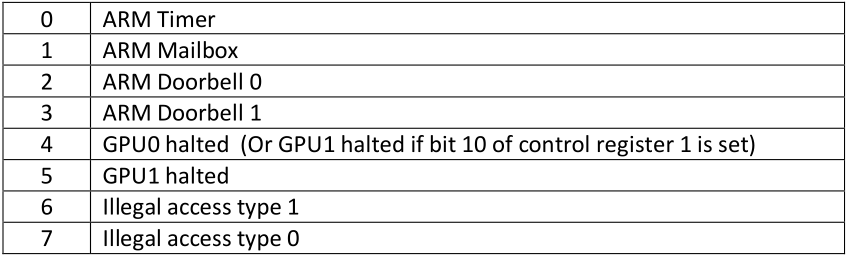
\includegraphics[scale=0.4]{figures/3-3.png}
\caption{ARM侧中断源}
\label{figure:3-3}
\end{figure}

\begin{figure}[htp]
\centering
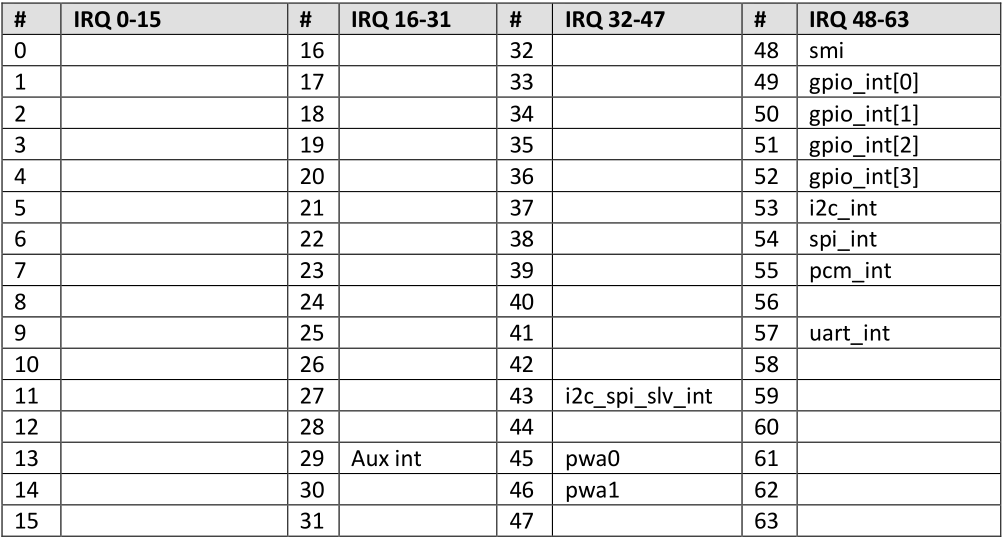
\includegraphics[scale=0.4]{figures/3-4.png}
\caption{GPU侧中断源}
\label{figure:3-4}
\end{figure}

我们按照先 ARM、后 GPU的顺序分配中断请求号码,即 ARM Timer的中断请求号码是0, ARM Mailbox是1, Illegal access type 0是7,然后 GPU的 IRQ 0-63对应于 8-71号。

\begin{code}
\captionof{listing}{chapter03/kernel/machdep.c}
\label{code:3-15}
\inputminted[firstline=91,lastline=125,linenos,numbersep=5pt,frame=lines,framesep=2mm]{c}{src/chapter03/kernel/machdep.c}
\end{code}

\noindent
其中 g\_\-intr\_\-vector是中断向量表,一个包含了 72个中断处理函数地址的数组。

\section{中断控制器}
中断控制器 (Programmable Interrupt Controller, PIC)是计算机重要的设备之一,它负责汇集所有外部设备的中断,然后把中断信号发送给 CPU,如图\ref{figure:3-5}所示。 CPSR中的I位控制着 CPU是否响应中断请求,而 PIC控制着每个设备的中断请求。

\begin{figure}[htp]
\centering
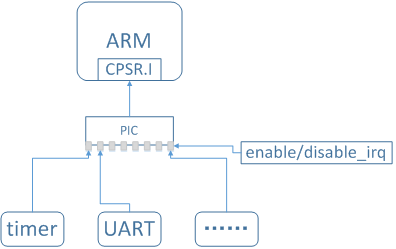
\includegraphics[scale=0.3]{figures/3-5}
\caption{中断控制器}
\label{figure:3-5}
\end{figure}

在系统启动过程中,要屏蔽所有设备的中断。这正是函数 init\_\-pic做的工作。

\begin{code}
\captionof{listing}{chapter03/kernel/machdep.c}
\label{code:3-16}
\inputminted[firstline=50,lastline=59,linenos,numbersep=5pt,frame=lines,framesep=2mm]{c}{src/chapter03/kernel/machdep.c}
\end{code}

将来某个设备初始化完成后,再逐一打开它的中断。控制 PIC中断开关的函数是 enable\_\-irq和 disable\_\-irq。

\begin{code}
\captionof{listing}{chapter03/kernel/machdep.c}
\label{code:3-17}
\inputminted[firstline=61,lastline=89,linenos,numbersep=5pt,frame=lines,framesep=2mm]{c}{src/chapter03/kernel/machdep.c}
\end{code}

\section{定时器中断}
可编程定时器 (Programmable Interval Timer,PIT)是整个系统的脉搏,驱动着系统推进各项工作。具体来说,它有两个作用:维持时钟和实现分时调度。定时器的工作方式比较简单,就是以固定的频率中断CPU。

\par
 BCM2835内部集成了一片定时器 AP804,下面我们对它进行初始化。定时器发出中断的频率可以修改,初始化定时器的函数 init\_\-pit的参数 freq,就是需要的中断频率。

\begin{code}
\captionof{listing}{chapter03/kernel/machdep.c}
\label{code:3-18}
\inputminted[firstline=127,lastline=142,linenos,numbersep=5pt,frame=lines,framesep=2mm]{c}{src/chapter03/kernel/machdep.c}
\end{code}

下面来实现定时器的中断处理函数。首先,我们定义了一个全局变量 g\_\-timer\_\-ticks记录定时器中断的次数。然后,为了验证定时器中断系统是否能工作,定时器中断一次,便往串口输出一个点。

\begin{code}
\captionof{listing}{chapter03/kernel/timer.c}
\label{code:3-19}
\inputminted[firstline=5,lastline=15,linenos,numbersep=5pt,frame=lines,framesep=2mm]{c}{src/chapter03/kernel/timer.c}
\end{code}

注意,在处理完中断后,要清除定时器的中断未决标志,表示本次中断处理完了,准备接收下一次中断。这个工作已经在 irq\_\-handler中完成了,见代码\ref{code:3-15}中的110-115行。

\par
现在,我们已经完成各个模块的工作,可以在 cstart函数中把它们组装起来。首先,初始化 PIC和 PIT,并把中断向量表填上默认的中断处理函数的地址。然后,把定时器中断处理函数的地址填入对应的中断向量表项,让 PIC开启定时器中断。最后,因为 CPU复位后默认不响应中断请求,即 CPSR.I=1,我们用函数 sti把 CPSR.I=0,即让 CPU响应中断请求。

\begin{code}
\captionof{listing}{chapter03/kernel/machdep.c}
\label{code:3-20}
\inputminted[firstline=144,lastline=176,linenos,numbersep=5pt,frame=lines,framesep=2mm]{c}{src/chapter03/kernel/machdep.c}
\end{code}

函数 sti和对应的关闭中断请求函数 cli定义在 entry.S中,如代码\ref{code:3-20}所示。

\begin{code}
\captionof{listing}{chapter03/kernel/entry.S}
\label{code:3-21}
\inputminted[firstline=155,lastline=168,linenos,numbersep=5pt,frame=lines,framesep=2mm]{gas}{src/chapter03/kernel/entry.S}
\end{code}

好了,代码写完了,回到命令行敲 make生成 kernel.img,把 kernel.img复制到 SD卡,插入树莓派并打开电源,在串口输出中可以看到树莓派正在打点,如图\ref{figure:3-6}所示。这说明中断系统已经可以工作了。

\begin{figure}[htp]
\centering
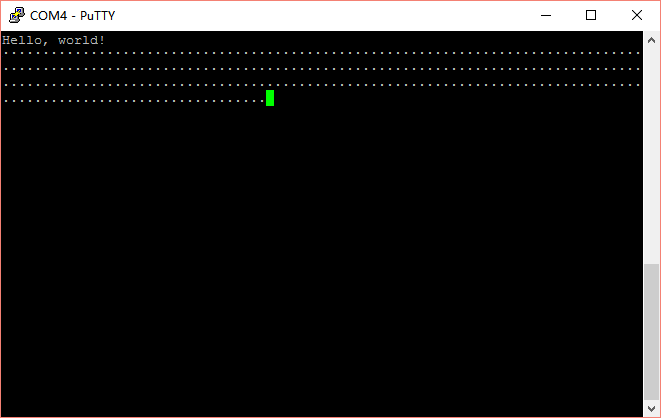
\includegraphics[scale=0.5]{figures/3-6.png}
\caption{定时器中断的输出}
\label{figure:3-6}
\end{figure}

\section{小结}
本章在第二章的基础上,加上了中断处理的功能,重点讲解了中断现场的保存与恢复。最后,以定时器中断为例子,演示了中断处理的流程。

\clearpage
\ifxetex\else\end{CJK*}\fi
\end{document} 